In chapter \ref{chap:application} we described the theoretical aspect behind our system. A software architecture was designed and the most significant scenarios was formalized and solved on a theoretical level. In this chapter we describe how we implemented the design into a application.    

%********************************************************************
\section{Introduction}
%********************************************************************
Implementing a software design can be a difficult task, as design modules rarely maps directly into code. Using the approach of different viewpoints and scenarios helps in this regard, but challenges due arise which could not have been foresee nor illustrate in the design phase. Challenges can come from our design of the development environment to the physical restricts of the deployment environment. 

%********************************************************************
\section{Method}
%********************************************************************
The final result is described in a top-down approach. We start with an informal description of the system, and from here gradually go into details starting with the module views which describes the static structures of the implementation. Then, follows the component and connector view to describe the dynamic structures. After the presentation of the implementation we will look at how choosen tactics have been implemented and how we solved the functional requirements of an electronic election.

%********************************************************************
\section{Development environment}
%********************************************************************
The implementation have been done using Microsoft ASP.NET framework, C\# and Javascript programming language. ASP.NET is a widely used and supported framework for creating web application. This framework is used both as the backend RESTful server, bulletin board and for the web server hosting the clients. The clients, voter and tallier is implemented using Javascript. Javascript have the benefits of running inside all modern browser and is widely used, thus giving us a very large set of libraries to our disposal. \\


\section{Final result}
In this section we describe the final implementation of the software design. 

%********************************************************************
\subsection{Overview}
%********************************************************************

\begin{figure}[H]
    \centering
    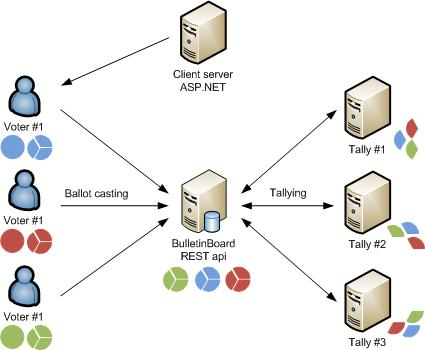
\includegraphics[scale=0.90]{Overview.jpg}
    \caption{Overview of the system}
    \label{fig:informal_overview}
\end{figure}

Figure \ref{fig:informal_overview} illustrates an overview of the system and the information flow in the different phases of the protocol. From left to right we see the voters each casting there votes and hiding their votes within a secret. Though secret sharing the vote is divided and encrypted into pieces corresponding to the number of talliers. The ballot casting phase ends with the voters publishing there votes and secret to the bulletin board. Ending the ballot casting phase starts the tallying phase where the talliers each collects there individual pieces of the secret, multiplying the shares together, decrypting the multiplum and publishes the decrypted multiplum to the bulletin board. The last segment of the tally phase, where the votes are calculated is not illustrated in the figure, but is none the less implemented by letting a dedicated tally do the calculating and posting the result to the bulletin board. \\

\noindent
The overview does not introduce many new elements to the implementation not previously known from the protocol, in fact the only new element introduced is the Client server which serves as a web-server for the voters, to which the voters logon in order to cast there votes. However the overview clearly shows the topology of the implementation, namely a star topology with a server (bulletin board) in the middle and Clients all around. There is no directly communication between the clients, all communication goes through the Server. This is due to the nature of an election, though we require the talliers to have a persistent connection to the server. We don't expect voters to stay connected throughout an entire election. The reason the bulletin board needs to have an persistent connection to the talliers is because after the ballot casting phase. The bulletin board needs to be able to notify the talliers for tallying phase.

%********************************************************************
\subsection{Viewpoints}
%********************************************************************
We use viewpoints as we further describes the implementation in details. We start with the module viewpoints which shows the static elements of the implementations, elements like packages, interfaces, classes and relations.

%********************************************************************
\subsubsection{Module view}
%********************************************************************
Starting from the top we look at how the implementation is structured into packages, where each packages contains elements that focuses on the same responsibility. Structuring our implementation this way follows the design principles of high cohesion and low coupling introduced in chapter \ref{chap:application} and lays the ground for code that is flexible and easily maintainable. 

\begin{figure}[H]
    \centering
    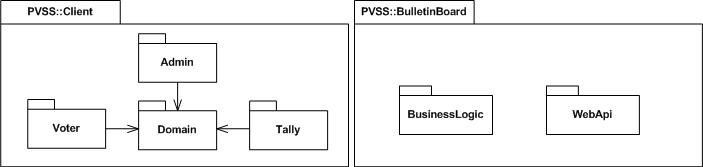
\includegraphics[scale=0.60]{Moduleview_packages_overview.jpg}
    \caption{Package overview}
    \label{fig:package_overview}
\end{figure}

\noindent
Figure \ref{fig:package_overview} shows a package overview of the entire implementation. The figure show both the packages included in the implementation of the Client and the bulletin board. The Client include packages containing logic specific for a Voter, Tally, Admin and the Domain package which holds logic used across the Client. The package overview of the bulletin board with only the two packages BusinessLogic and WebApi looks on the surface very simply, but below we unfold each package showing a more complex structure. 

\begin{figure}[H]
    \centering
    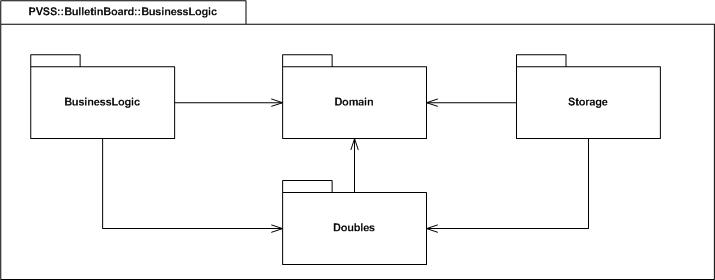
\includegraphics[scale=0.60]{Moduleview_packages_BulletinBoard.jpg}
    \caption{Package overview of bulletin board business logic}
    \label{fig:package_overview_of_bulletinboard_businesslogic}
\end{figure}

\noindent
Figure \ref{fig:package_overview_of_bulletinboard_businesslogic} shows the packages revealed when unfolding the BusinessLogic package. This include the sub-packages BusinessLogic, Storage, Doubles and Domain. The packages BusinessLogic, Storage and Domain is fairly self explanatory. The package Double holds the logic we used in order to unit test our implementation. \\


\begin{figure}[H]
    \centering
    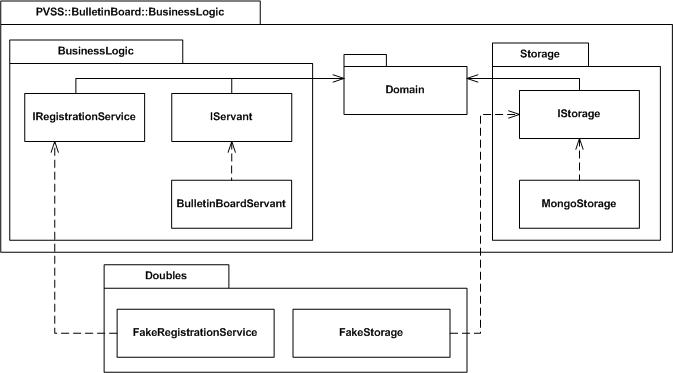
\includegraphics[scale=0.60]{Moduleview_Class.jpg}
    \caption{Module view of bulletin board}
    \label{fig:module_over_of_bulletinboar}
\end{figure}

\noindent
Figure \ref{fig:module_over_of_bulletinboar} shows the interfaces and classes within the BusinessLogic package of the bulletin board. Note that the package Doubles have been left outside the container of the BusinessLogic, this is due to the fact that its responsibilities only evolves around testing and the packages is not used in the production environment. Also noticeable is the Domain package have not been specified further. The reason for this is, that it simply holds the representation of physical elements like a ballot, a voter, a share etc, which contain no business logic.

\begin{description}
    \item[IRegistrationService] is an interface that holds the responsibility of the \textit{Registration authority} specified in section \ref{sec:the_voting_process}. Is validates and registries eligible voters.  For this implementation we only included the class \textbf{FakeRegistrationService} which implements responsibilities from the IRegistrationService. 
    
    \item[IServant] is an interface that have the responsibilities of the \textit{bulletin board} also the described in section \ref{sec:the_voting_process}. It handles the communication with the Clients and insures the persistence of the election data such as the ballots and shares etc. The class \textbf{BulletinBoardServant} implements the responsibilities of the IServant. A key functionality of the BulletinBoardServant is that most of its methods is read-only, this helps to ensure that no honest or dishonest user removes information. 
    
    \item[IStorage] is an interface that have the responsibilities of persisting and retrieving data. Both the classes \textbf{MongoStorage} and \textbf{FakeStorage} implements the responsibilities of the IStorage. The \textbf{MongoStorage} also acts as a client to a Mongo database to which it stores the data, where the \textbf{FakeStorage} simply stores the data in memory, meaning that the data is lost when the application stops. 
    
\end{description}

\begin{figure}[H]
    \centering
    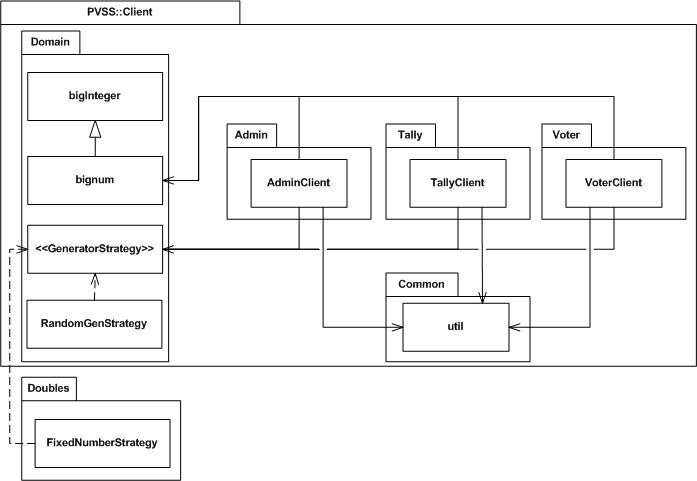
\includegraphics[scale=0.60]{Moduleview_Class_Client.jpg}
    \caption{Module view of Client}
    \label{fig:module_view_of_client}
\end{figure}

\noindent
Figure \ref{fig:module_view_of_client} shows the interfaces and classes of the Client. Again the package Double is left outside the content of the Client, due to the same arguments stated above. 

\begin{description}
    \item[util] is a simple class that holds some helper function, that is used across the system. 
    
    \item[bignum] is a class that inherits the functionlitites from its superclass \textbf{bigInteger}. This structure enables us to expand or alter the functionalities of the \textbf{bigInteger} without changing the class. 
    
    \item[INumberGenerator] is an interface which have the responsibility of generating random integers and primes. The classes \textbf{RandomGenStrategy} and \textbf{FixedNumberStrategy} both implements the responsibilities of INumberGenerator. \textbf{FixedNumberGenerator} is used for testing and enabling us to control the numbers return. 

    \item[AdminClient] is a class that holds the responsibilities of creating an election and generating the public elements used in the election. The AdminClient is depending on the class Bignum, and the Interface INumberGenerator. 
    
    \item[VoterClient] is a class that holds the responsibilities of a \textit{Voter} described in the protocol, section ~\ref{sec:ballot_casting}. This class, like the AdminClient is depending on Bignum and INumberGenerator.    
    
    \item[TallyClient] is a class that holds the responsibilities of a \textit{Tally} described in the protocol, section ~\ref{sec:tallying}. This class, is also depending on the Bignum and INumberGenerator. 
\end{description}

\noindent
This last module view concludes the overall static structure of the implementation, we however have not further specified the elements in the Webapi package shown in figure \ref{fig:package_overview}. The reason for this, is that it does not hold any elements related to the protocol but only elements regarding the implementation of the REST interface describe in the Interoperability tactic in section \ref{sec:interoperability:restapi} and this implementation is discussed later. \\

%********************************************************************
\subsubsection{Component and Connector view}
%********************************************************************
For this next part we will look at how the dynamic components in the implementation interacts during runtime. We will present an overall insight of the system's interaction. 

\begin{figure}[H]
    \centering
    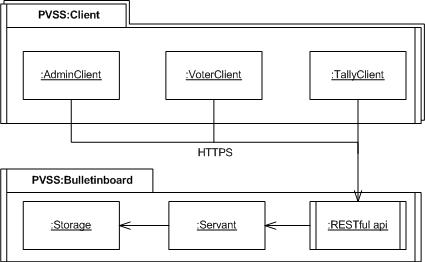
\includegraphics[scale=.7]{CC_Overall_View.jpg}
    \caption{Overall Component and Connector view}
    \label{fig:CC_overall_View}
\end{figure}

\noindent
Figure \ref{fig:CC_overall_View} shows how the system interact overall. As we have seen in the module views, there is no interacting between the components in the Client. They each operates independently and they all communicates with the bulletin board through the REST API.  The communication between the Clients and the bulletin board is done through an HTTPS connection. This connection uses Secure Socket Layer (SSL) or Transport Layer Security (TLS) to encrypt the messages sent or received. All successful communication done with the REST API is forward to the Servant component that handles the business logic. If there is a need for persisting data, then the Servant sends the data to the Storage. \\

\noindent
The following sequence diagram shows the overall flow of the system from the ballot casting phase to the result. The internal method calls and calculations done on each individual class is not show, in order to present a better overview.  

\begin{figure}[H]
    \centering
    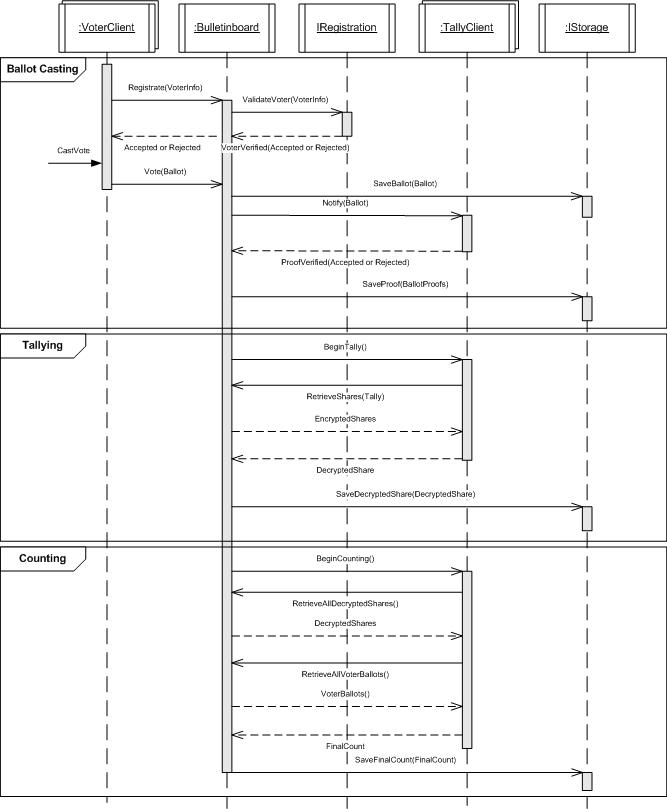
\includegraphics[scale=.7]{CC_SekvensDiagram.jpg}
    \caption{Overall Sequence diagram}
    \label{fig:CC_sequence_diagram}   
\end{figure}

%********************************************************************
\subsubsection{Allocation view}
%********************************************************************
Finishing out the viewpoints we lastly have a deployment view showing the systems requirements to the deployment environment. 

\begin{figure}[H]
    \centering
    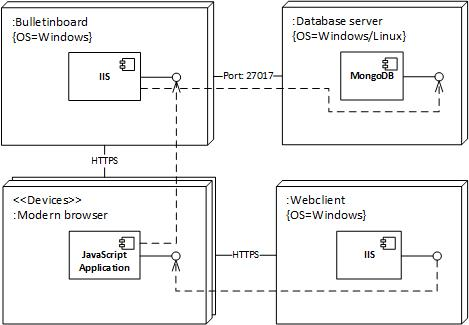
\includegraphics[scale=.7]{deployment_view.jpg}
    \caption{Final deployment view}
    \label{fig:final_deployment_view}
\end{figure}

\noindent
Figure \ref{fig:final_deployment_view} shows that the system requires three servers, a database server running a mongo database, a web-server with a Internet Information Server (IIS) installed to host the bulletin board RESTful Webapi and lastly a web-server also with IIS installed to host the Webclient. We also require that devices that is to communicate with the system needs to have a modern browser installed, that is able to execute Javascripts. 


%********************************************************************
\section{Implementing the tactics}
%********************************************************************
In this section we will highlight selected implementation of previously described tactics from chapter \ref{chap:application}.

%********************************************************************
\subsection{Interoperability: REST API}
%********************************************************************
As stated earlier we use a REST interface which should be easily accessible by everyone. This means that our bulletin board is build on some of the REST principles. Figure \ref{fig:rest_electronic_voting_web_service_model} illustrate an informal webservice model which describes our resources on the bulletin board. The process of constructing this diagram gives overview and insight of how we could design a REST interface on the different resources. 

\begin{figure}[H]
    \centering
     \makebox[\textwidth]{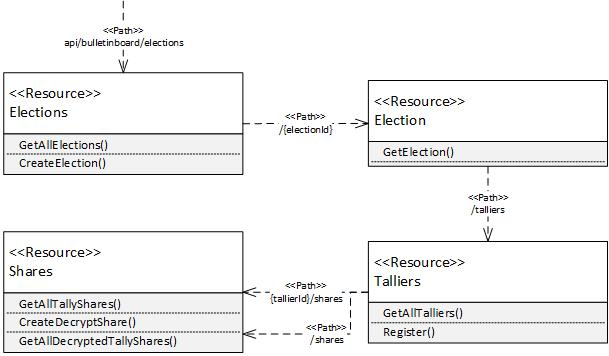
\includegraphics[scale=0.60]{rest-classdiagram.jpg}}
     \caption{Overview of REST electronic voting web service model}
     \label{fig:rest_electronic_voting_web_service_model}
\end{figure}


\noindent
Figure \ref{fig:rest_api_to_the_Bulletinboard} shows our final REST api. The urls shows how the REST api can be accessed together with the HTTP methods which shows which methods can be invoked on the different urls. 


\begin{table}[H]\fontsize{8}{9}\selectfont
\centering
\begin{tabular}{|l|l|l|}
\hline
Resource                                                    & URL                                                & HTTP methods                                                            \\ \hline
Elections                                                   & /elections                                         & \begin{tabular}[c]{@{}l@{}}GET GetAllElections\\ POST CreateElection\end{tabular} \\ \hline
Election                                                    & /elections/\{electionId\}                                  & GET GetElection                                                                   \\ \hline
Votes                                                       & /elections/\{id\}/votes                            & \begin{tabular}[c]{@{}l@{}}GET GetAllVotes\\ POST CreateVote\end{tabular}         \\ \hline
Talliers                                                    & /elections/\{id\}/talliers                         & \begin{tabular}[c]{@{}l@{}}GET GetAllTalliers\\ POST Register\end{tabular}        \\ \hline
Shares                                                      & /elections/\{id\}/talliers/\{id\}/shares           & \begin{tabular}[c]{@{}l@{}}GET GetAllTallyShares \\  POST CreateDecryptShare     \end{tabular}                                                            \\ \hline
\begin{tabular}[c]{@{}l@{}}Decrypted \\ shares\end{tabular} & /elections/\{id\}/talliers/shares        & \begin{tabular}[c]{@{}l@{}}GET GetAllDecrypted\\ TallyShares\end{tabular}                                                        \\ \hline
\end{tabular}
\caption{REST api to the bulletin board}
\label{fig:rest_api_to_the_Bulletinboard}
\end{table}


\noindent
Since our webclients is build purely on Javascript, all communication is done through ajax call to the bulletin board. Listings \ref{lst:javascript_rest_api} illustrates how one can interact with REST api. The example shows how to create an election. This is called by the Admin client which starts the election.   \\ 


\begin{lstlisting}[language=Javascript, caption=Javascript example, label=lst:javascript_rest_api]
    $.ajax({
        type: "POST",
        url: "api/bulletinboard/elections",
        data: jsonData,
        success: function (data) {
            if (callBack)
                callBack(data);
        },
        contentType: "application/json"
    });
\end{lstlisting}


 
%********************************************************************
\subsection{Modifiability: Number generator}
%******************************************************************** 
Implementing this tactic proved to be fairly easy. However as the dynamic nature of Javascript does not support the concept
of interfaces as we know it from Java and C\#, we had to introduce a method to secure that the injected NumberGenerator strategy
applies to its responsibilities. To construct this method we utilizes the concept of \textit{Duck Typing} which basically states that
if an object walks like a duck and quarks like a duck, then to the concerns of Javascript it is a duck!. 

\begin{lstlisting}[language=Javascript, caption=Implementation of Duck typing, label=lst:ducktyping]
    // example duck typing method
    var InterfaceMethods = function (obj /*, method list as strings */) {
        var i = 1, methodName;
        while ((methodName = arguments[i++])) {
            if (typeof obj[methodName] != 'function') {
                return false;
            }
        }
        return true;
    }
\end{lstlisting}

\noindent
In the following listing \ref{lst:interface_randgen} we show how the InterfaceMethod method is used to check
for an interface object. It checks if the methods specified in the parameters is to be found on the object passed as the 
first parameter. In the example below it checks for the methods "randBetween" and "randPrimeBetween".

\begin{lstlisting}[language=Javascript, caption=Checking for an interface, label=lst:interface_randgen]
var voterClient = function (serv, options) {
    ...
    ...
    var randomGen;                     

    if (options) {
        if (options.randomGen) {
            if (util.InterfaceMethods(options.randomGen, 'randBetween', 'randPrimeBetween')) {
                randomGen = options.randomGen;
            }
        }
    } 
\end{lstlisting}
 
\noindent
As shown in the listing \ref{lst:interface_randgen} the NumberGenerator strategy is simply injected
into the VoterClient upon creation. Methods within the VoterClient can now execute the methods
randBetween and randPrimeBetween on the injected object through the variable randomGen. 
 
 


%********************************************************************
\section{Analyzing the application}
%********************************************************************
In this section we will list the security requirements from section \ref{sec:security_requirements}.  We will then evaluate these requirements against our application. 

%********************************************************************
\subsection{Electronic voting secure requirements} \label{sec:analyzing_electronic_voting_secure_requirements}
%********************************************************************
\begin{description}
    \item[Voter Privacy]
        \textit{No one should be able to link a vote back to the specific voter, and only the voter should
        know his vote. These requirements shall hold during and after the election.}  
        
        This requirement is meet by our implementation, infact its one of the core elements in the
        election voting protocol from section \ref{sec:the_protocol}. Every voter only publish his vote
        though $U = G^{v+s}$ where $G$ is a generator and $v \in \{0,1\}$ and $s \in \Z_q$. As $s$ is only
        known by the voter and is uniformly random picked then the sum of $s$ and $v$ is also unknown for any 
        potential adversary under the security of the DL problem. And one could ague that even if an
        adversary should be break the DL problem then, unless he knows $s$, the vote $v$ would still
        be unknown.
        
    \item[Eligibility]
        \textit{Only Eligible and registered voters can vote.}    
        
        Unlike Voter Privacy, this requirement of non-eligible voters not being able to vote is not
        fulfill by the protocol it self. First we need a list of eligible voters which acts as a reference list for which voter are allowed to vote. Second our registration service handles registration which is described in
        section  \ref{sec:modifiability_registations_process}. This enable us to change the registration service 
        accordingly to the nature of the election.   
      
        
    \item[Uniqueness]
        \textit{Only one vote per registered voter should be counted.}
        
        Uniqueness is about making sure only one vote is counted for each eligible
        voter. This requirement is meet by having a separate table in the database with all eligible voters 
        containing an id and a 0/1 (no or yes). This table will be updated when votes arrive to the bulletin board. 
        
    \item[Fairness]
        \textit{None should be able to gain any knowledge of the outcome of the election, before the ending. This is to prevent voters of voting accordingly to any leaked information.}       
    
        This is achieved in our implementation by only starting the tally phase when all votes are casted or when a deadline is 
        reached and the ballot casting phase ends. Only the bulletin board have the authority to notify the talliers when to begin the tallying phase.  
        
        Through the property of secret sharing used in the protocol, the secret to decrypt the
        vote is shared amoungst three or more talliers. These shares are again encrypted with the public key 
        of the corresponding tally. As a consequence, no one except the tally with the corresponding
        private key is able to decrypt the share.
  
           
    \item[Uncoercibility] 
        \textit{Nobody should be able to extract the value of a vote. This is to prevent anybody from compelling a voter by force, intimidation, or authority to cast a vote in a specific way.}
    
        Since our application is classified as a \textit{remote internet voting} described in section \ref{sec:voting:classification}, we are not able to control the physical environments to where the votes are casted. Therefor we are not able to fulfill this requirement to its fullest. However the protocol ensure that no coercer is able to extract a specific value of a vote, due to properties already mentioned in the previous requirements.         
        
    \item[Receipt-freeness] 
        \textit{The voting system should not produce a receipt that reveals any information about the casted vote. This is to prevent a voter from trading his vote.}
            
        Our application only confirms the success of a voting, not the value of the vote. There is no functionality that enables any  participants nor observers to gain information about the value of a vote.         
        
    \item[Accuracy]
        \textit{The final tally should be correctly computed from valid casted votes. It should not be possible to manipulate the final tally without being detected.}
        
        \noindent
        Our implementation utilizes the proofs from the protocol to fulfill this requirement. 
        
        \noindent
        Under the ballot casting phase of the protocol, we require that the voters proofs the correctness of there votes. This is done through the $Proof_U$ and $DLEQ$ proofs, which is required to be published along side the encrypted vote $U$. Should one of the proofs fail, then the vote is marked invalid and this vote is ignore in the preceding processes. 
        
        \noindent
        In the tally phase of the protocol, the tally multiplies its shares and then decrypts them and publishes the end result. Along with this result we require that the $DLEQ$ proof is published aswell. This allows us to verify the correctness of the tallying process for each tally. Should a $DLEQ$ proof from a tally fail then the tally's shares is ignored in the preceding process. The protocol requires the shares from at least $t$ talliers, in order to extract and calculate the end result. Should it 
        be the case that this requirement is not fulfill an re-election is require but untill then the implementation simply ignores the shares from the tally in question.
        
        \noindent
        Should an adversary gain access to the database serving the bulletin board, it would be possible for this adversary to manipulate the verdict of a proof but not
        the proofs them self, as the construction of the proofs prevent this. Though our application does not take this scenario into account it would be fairly easy to make
        a functionality that reevaluates the proofs, should such a breach have been detected. One could argue that an adversary with full access to the database could also remove elements such as a casted vote or the information that a given voter have voted. The later would effectually enable the given voter the ability to double vote. This scenario is not handled in our application. The first scenario is also possible but given the fact that our application have voter privacy and the votes is secure under the DL problem then the adversary would not know if he is removing and "no" or a "yes" vote. 
        
        
    \item[Universal Verifiability]
        \textit{It should be possible for any participants and observers to validate individual votes as well as the final tally of the election.}
        
        \noindent
        The protocol is basically designed around this requirement as voters publishes their ballot and proofs to the bulletin board. The Tally will also publish a proof under the tallying phase. Any participant or observers can validate the proofs since it is public. 
        
        
        \noindent
        Everything on the bulletin board is publicly available both for participants and none participants of the election. $Proof_U$ verifies that an encrypted vote $U$ is either 0 or 1 and the $DLEQ$ proofs verifies the consistence of the shares for both the voters and the talliers. The end result can be calculated from the publicly known information available after the tallying phase. 
            
    \item[Individual Verifiability]
        \textit{Every registered voter should be able to verify that his vote is counted correctly.}
        
        This requirement is contradicting with the requirement of receipt-freeness. The challenge is how can one voter verify that his vote 
        is calculated and included in the final tally correctly. This can not be done directly - however we state with the following two new informal requirements, every votes is calculated and included in the final tally and as such his vote is calculated and included correctly.
        \begin{enumerate}
            \item All votes from the ballot casting is included in the final tally.
            \item Every vote from the ballot casting is calculated correctly.
        \end{enumerate}
        
        \noindent        
        With the protocol we can fulfill these two requirements. However we have not implemented the necessary functionality in the application.  We will elaborate on these two statements under the discussion section \ref{sec:discussion_individual_verifiability}. 
        
    \end{description}

